

\tikzset{every picture/.style={line width=0.75pt}} %set default line width to 0.75pt        

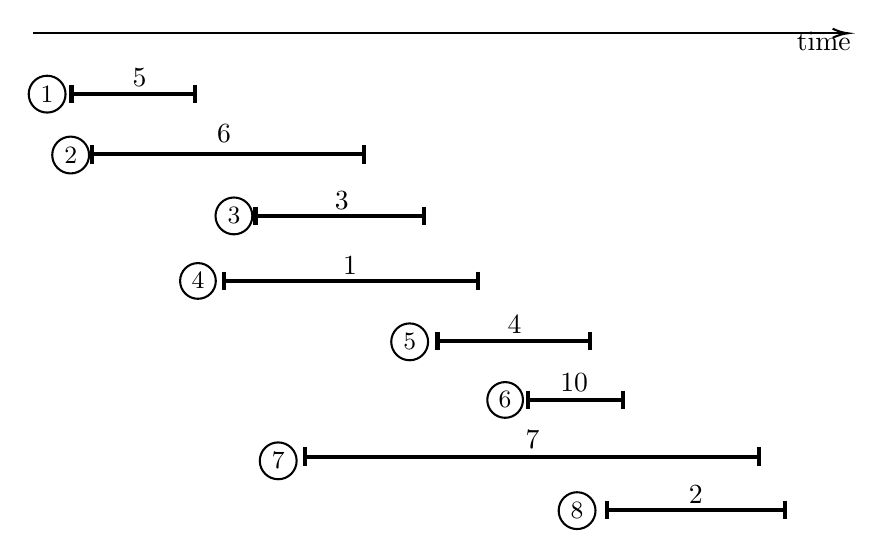
\begin{tikzpicture}[x=0.5pt,y=0.5pt,yscale=-1,xscale=1]
%uncomment if require: \path (0,383); %set diagram left start at 0, and has height of 383

%Straight Lines [id:da9015649955021968] 
\draw    (5,13) -- (592,13) ;
\draw [shift={(594,13)}, rotate = 180] [color={rgb, 255:red, 0; green, 0; blue, 0 }  ][line width=0.75]    (10.93,-3.29) .. controls (6.95,-1.4) and (3.31,-0.3) .. (0,0) .. controls (3.31,0.3) and (6.95,1.4) .. (10.93,3.29)   ;
%Straight Lines [id:da9640237890291299] 
\draw [line width=1.5]    (33,57) -- (122.5,57) ;
\draw [shift={(122.5,57)}, rotate = 180] [color={rgb, 255:red, 0; green, 0; blue, 0 }  ][line width=1.5]    (0,6.71) -- (0,-6.71)   ;
\draw [shift={(33,57)}, rotate = 180] [color={rgb, 255:red, 0; green, 0; blue, 0 }  ][line width=1.5]    (0,6.71) -- (0,-6.71)   ;
%Straight Lines [id:da3355888679808179] 
\draw [line width=1.5]    (166,145) -- (287.5,145) ;
\draw [shift={(287.5,145)}, rotate = 180] [color={rgb, 255:red, 0; green, 0; blue, 0 }  ][line width=1.5]    (0,6.71) -- (0,-6.71)   ;
\draw [shift={(166,145)}, rotate = 180] [color={rgb, 255:red, 0; green, 0; blue, 0 }  ][line width=1.5]    (0,6.71) -- (0,-6.71)   ;
%Straight Lines [id:da09988799250468405] 
\draw [line width=1.5]    (363,278) -- (431.5,278) ;
\draw [shift={(431.5,278)}, rotate = 180] [color={rgb, 255:red, 0; green, 0; blue, 0 }  ][line width=1.5]    (0,6.71) -- (0,-6.71)   ;
\draw [shift={(363,278)}, rotate = 180] [color={rgb, 255:red, 0; green, 0; blue, 0 }  ][line width=1.5]    (0,6.71) -- (0,-6.71)   ;
%Straight Lines [id:da4026459071674142] 
\draw [line width=1.5]    (48,100.5) -- (244.5,100.5) ;
\draw [shift={(244.5,100.5)}, rotate = 180] [color={rgb, 255:red, 0; green, 0; blue, 0 }  ][line width=1.5]    (0,6.71) -- (0,-6.71)   ;
\draw [shift={(48,100.5)}, rotate = 180] [color={rgb, 255:red, 0; green, 0; blue, 0 }  ][line width=1.5]    (0,6.71) -- (0,-6.71)   ;
%Straight Lines [id:da5509115882034084] 
\draw [line width=1.5]    (297.5,235.5) -- (407.5,235.5) ;
\draw [shift={(407.5,235.5)}, rotate = 180] [color={rgb, 255:red, 0; green, 0; blue, 0 }  ][line width=1.5]    (0,6.71) -- (0,-6.71)   ;
\draw [shift={(297.5,235.5)}, rotate = 180] [color={rgb, 255:red, 0; green, 0; blue, 0 }  ][line width=1.5]    (0,6.71) -- (0,-6.71)   ;
%Straight Lines [id:da6271509388583772] 
\draw [line width=1.5]    (420,357.5) -- (548.5,357.5) ;
\draw [shift={(548.5,357.5)}, rotate = 180] [color={rgb, 255:red, 0; green, 0; blue, 0 }  ][line width=1.5]    (0,6.71) -- (0,-6.71)   ;
\draw [shift={(420,357.5)}, rotate = 180] [color={rgb, 255:red, 0; green, 0; blue, 0 }  ][line width=1.5]    (0,6.71) -- (0,-6.71)   ;
%Straight Lines [id:da26802882985941956] 
\draw [line width=1.5]    (143.5,192) -- (327,192) ;
\draw [shift={(327,192)}, rotate = 180] [color={rgb, 255:red, 0; green, 0; blue, 0 }  ][line width=1.5]    (0,6.71) -- (0,-6.71)   ;
\draw [shift={(143.5,192)}, rotate = 180] [color={rgb, 255:red, 0; green, 0; blue, 0 }  ][line width=1.5]    (0,6.71) -- (0,-6.71)   ;
%Straight Lines [id:da22029647624095072] 
\draw [line width=1.5]    (201.5,319) -- (530,319) ;
\draw [shift={(530,319)}, rotate = 180] [color={rgb, 255:red, 0; green, 0; blue, 0 }  ][line width=1.5]    (0,6.71) -- (0,-6.71)   ;
\draw [shift={(201.5,319)}, rotate = 180] [color={rgb, 255:red, 0; green, 0; blue, 0 }  ][line width=1.5]    (0,6.71) -- (0,-6.71)   ;

% Text Node
\draw (555,10) node [anchor=north west][inner sep=0.75pt]   [align=left] {time};
% Text Node
\draw    (15.38, 57) circle [x radius= 13.31, y radius= 13.31]   ;
\draw (15.38,57) node  [font=\small] [align=left] {$\displaystyle 1$};
% Text Node
\draw    (150.38, 145) circle [x radius= 13.31, y radius= 13.31]   ;
\draw (150.38,145) node  [font=\small] [align=left] {$\displaystyle 3$};
% Text Node
\draw    (346.38, 278) circle [x radius= 12.9, y radius= 12.9]   ;
\draw (346.38,278) node  [font=\small] [align=left] {6};
% Text Node
\draw    (32.38, 101) circle [x radius= 13.31, y radius= 13.31]   ;
\draw (32.38,101) node  [font=\small] [align=left] {$\displaystyle 2$};
% Text Node
\draw    (277.38, 236) circle [x radius= 13.31, y radius= 13.31]   ;
\draw (277.38,236) node  [font=\small] [align=left] {$\displaystyle 5$};
% Text Node
\draw    (398.38, 358) circle [x radius= 13.31, y radius= 13.31]   ;
\draw (398.38,358) node  [font=\small] [align=left] {$\displaystyle 8$};
% Text Node
\draw    (124.38, 192) circle [x radius= 12.9, y radius= 12.9]   ;
\draw (124.38,192) node  [font=\small] [align=left] {4};
% Text Node
\draw    (182.38, 322) circle [x radius= 13.31, y radius= 13.31]   ;
\draw (182.38,322) node  [font=\small] [align=left] {$\displaystyle 7$};
% Text Node
\draw (75,36) node [anchor=north west][inner sep=0.75pt]   [align=left] {$\displaystyle 5$};
% Text Node
\draw (221,125) node [anchor=north west][inner sep=0.75pt]   [align=left] {$\displaystyle 3$};
% Text Node
\draw (384,257) node [anchor=north west][inner sep=0.75pt]   [align=left] {$\displaystyle 10$};
% Text Node
\draw (136,77) node [anchor=north west][inner sep=0.75pt]   [align=left] {$\displaystyle 6$};
% Text Node
\draw (346,215) node [anchor=north west][inner sep=0.75pt]   [align=left] {$\displaystyle 4$};
% Text Node
\draw (477,338) node [anchor=north west][inner sep=0.75pt]   [align=left] {$\displaystyle 2$};
% Text Node
\draw (227,172) node [anchor=north west][inner sep=0.75pt]   [align=left] {$\displaystyle 1$};
% Text Node
\draw (359,298) node [anchor=north west][inner sep=0.75pt]   [align=left] {$\displaystyle 7$};


\end{tikzpicture}

